%% LyX 2.0.4 created this file.  For more info, see http://www.lyx.org/.
%% Do not edit unless you really know what you are doing.
\documentclass[english,letterpaper, 10 pt, conference]{ieeeconf}
\usepackage[T1]{fontenc}
\usepackage[latin9]{inputenc}
\usepackage{listings}
\usepackage{prettyref}
\usepackage{float}
\usepackage{amsmath}
\usepackage{graphicx}
\usepackage{xargs}[2008/03/08]

\makeatletter

%%%%%%%%%%%%%%%%%%%%%%%%%%%%%% LyX specific LaTeX commands.
%% A simple dot to overcome graphicx limitations
\newcommand{\lyxdot}{.}

\floatstyle{ruled}
\newfloat{algorithm}{tbp}{loa}
\providecommand{\algorithmname}{Algorithm}
\floatname{algorithm}{\protect\algorithmname}

%%%%%%%%%%%%%%%%%%%%%%%%%%%%%% Textclass specific LaTeX commands.
\newtheorem{example}{Example}
\newtheorem{definitn}{Definition}
\newtheorem{lemma}{Lemma}
\newtheorem{cor}{Corollary}
\newtheorem{prop}{Proposition}
\newtheorem{case}{Case}
\newtheorem{thm}{Theorem}

%%%%%%%%%%%%%%%%%%%%%%%%%%%%%% User specified LaTeX commands.

\IEEEoverridecommandlockouts                              % This command is only
                                                          % needed if you want to
                                                          % use the \thanks command
\overrideIEEEmargins
% See the \addtolength command later in the file to balance the column lengths
% on the last page of the document

\@ifundefined{showcaptionsetup}{}{%
 \PassOptionsToPackage{caption=false}{subfig}}
\usepackage{subfig}
\makeatother

\usepackage{babel}
\begin{document}
\global\long\def\vect#1{\boldsymbol{#1}}
 \global\long\def\lonenorm#1{\left|\left|#1\right|\right|_{1}}
\global\long\def\dotT#1#2{\vect{#1^{\mathrm{T}}} \vect{#2} }


\newcommandx\mass[1][usedefault, addprefix=\global, 1=]{\rho_{#1}}
 \newcommandx\massmax[1][usedefault, addprefix=\global, 1=]{\mass[#1]^{\max}}
 \newcommandx\masscrit[1][usedefault, addprefix=\global, 1=]{\mass[#1]^{\text{crit}}}
\global\long\def\vmass{\vect{\mass}}


\global\long\def\Junctions{V}
 \global\long\def\Cells{E}
 \global\long\def\Graph{(\Junctions,\Cells)}


\newcommandx\junction[1][usedefault, addprefix=\global, 1=]{v_{#1}}
 \newcommandx\jcn[1][usedefault, addprefix=\global, 1=]{\junction[#1]}


\newcommandx\cell[1][usedefault, addprefix=\global, 1=]{e_{#1}}
 \newcommandx\vcell[1][usedefault, addprefix=\global, 1=]{\vect{\cell[#1]}}


\global\long\def\Incoming{I}
 \newcommandx\inCells[1][usedefault, addprefix=\global, 1=]{\Incoming_{#1}}


\global\long\def\Outgoing{O}
 \newcommandx\outCells[1][usedefault, addprefix=\global, 1=]{\Outgoing_{#1}}


\global\long\def\speedff{v^{f}}
\global\long\def\speedCong{v^{c}}


\global\long\def\minify#1{#1^{\text{min}}}
 \global\long\def\maxify#1{#1^{\text{\ensuremath{\max}}}}
 \global\long\def\inify#1{#1^{\text{in}}}
 \global\long\def\outify#1{#1^{\text{out}}}


\newcommandx\flow[1][usedefault, addprefix=\global, 1=]{x_{#1}}
 \newcommandx\flowMax[1][usedefault, addprefix=\global, 1=]{\maxify{\flow[#1]}}
 \newcommandx\flowIn[1][usedefault, addprefix=\global, 1=]{\inify{\flow[#1]}}
 \newcommandx\flowOut[1][usedefault, addprefix=\global, 1=]{\outify{\flow[#1]}}


\global\long\def\vflow{\vect q}
 \global\long\def\vflowMax{\maxify{\vect{\flow}}}
 \global\long\def\vflowIn{\inify{\vect{\flow}}}
 \global\long\def\vflowOut{\outify{\vect{\flow}}}


\newcommandx\demand[1][usedefault, addprefix=\global, 1=]{\Delta_{#1}}
 \newcommandx\dem[1][usedefault, addprefix=\global, 1=]{\demand[#1]}
 \newcommandx\supply[1][usedefault, addprefix=\global, 1=]{\Sigma_{#1}}
 \newcommandx\supp[1][usedefault, addprefix=\global, 1=]{\supply[#1]}


\global\long\def\fa#1{\forall\,#1}
 \global\long\def\fain#1#2{\fa{#1\,\in\,#2}}


\newcommandx\totaltraveltime[1][usedefault, addprefix=\global, 1=]{TTT_{#1}}
 \newcommandx\ttt[1][usedefault, addprefix=\global, 1=]{\totaltraveltime[#1]}


\newcommandx\qdemand[1][usedefault, addprefix=\global, 1=]{r_{#1}}


\newcommandx\delay[1][usedefault, addprefix=\global, 1=]{D_{#1}}


\newcommandx\lenCell[1][usedefault, addprefix=\global, 1=]{L_{#1}}


\newcommandx\Rea[1][usedefault, addprefix=\global, 1=]{\mathcal{R}^{#1}}


\newcommandx\Routes[1][usedefault, addprefix=\global, 1=]{R_{#1}}


\global\long\def\cellRoute#1#2{\gamma_{#1.#2}}
\global\long\def\odRoute#1#2{\psi_{#1.#2}}


\global\long\def\degradeRatio{}




\renewcommandx\mass[1][usedefault, addprefix=\global, 1=]{\rho_{#1}}
 \renewcommandx\massmax[1][usedefault, addprefix=\global, 1=]{\mass[#1]^{\max}}
 \renewcommandx\masscrit[1][usedefault, addprefix=\global, 1=]{\mass[#1]^{\text{crit}}}
\global\long\def\vmass{\vect{\mass}}


\renewcommandx\qdemand[1][usedefault, addprefix=\global, 1=]{r_{#1}}


\renewcommandx\flow[1][usedefault, addprefix=\global, 1=]{x_{#1}}
 \renewcommandx\flowMax[1][usedefault, addprefix=\global, 1=]{\maxify{\flow[#1]}}
 \renewcommandx\flowIn[1][usedefault, addprefix=\global, 1=]{\inify{\flow[#1]}}
 \renewcommandx\flowOut[1][usedefault, addprefix=\global, 1=]{\outify{\flow[#1]}}




\global\long\def\Network{\mathscr{N}}
\global\long\def\NLinks{N}
\global\long\def\Graph{G}


\newcommandx\Mode[1][usedefault, addprefix=\global, 1=]{m_{#1}}


\newcommandx\latency[1][usedefault, addprefix=\global, 1=]{l_{#1}}
\global\long\def\Latency{C}


\global\long\def\link{n}


\newcommandx\Length[1][usedefault, addprefix=\global, 1=]{\lenCell[#1]}


\newcommandx\cFlow[1][usedefault, addprefix=\global, 1=]{s_{#1}}
\newcommandx\ncFlow[1][usedefault, addprefix=\global, 1=]{t_{#1}}


\newcommandx\parA[1][usedefault, addprefix=\global, 1=]{a_{#1}}
\newcommandx\parB[1][usedefault, addprefix=\global, 1=]{b_{#1}}
\newcommandx\parC[1][usedefault, addprefix=\global, 1=]{c_{#1}}


\global\long\def\coloneqq{:=}




\global\long\def\BestNashEquilibrium#1#2{\textup{BNE}\left(#1,#2\right)}
\global\long\def\NashEquilibrium#1#2#3{\textup{NE}_{#3}\left(#1,#2\right)}




\global\long\def\cffFlow#1#2{\hat{\flow}_{#1}\left(#2\right)}




\newcommandx\opneFlow[3][usedefault, addprefix=\global, 1=]{\bar{\flow}_{#1}^{#2,#3}}




\newcommandx\cffMode[2][usedefault, addprefix=\global, 1=]{\bar{\Mode}_{#1}^{#2}}


\global\long\def\Supp#1{\textup{Supp}\left(#1\right)}


\global\long\def\POS#1#2{\textup{POS}\left(#1,#2\right)}


\global\long\def\Cost#1#2{C_{#1}\left(#1,#2\right)}


\global\long\def\compRate{\alpha}


\global\long\def\StackSet{\textup{S}(\NLinks,\qdemand,\compRate)}


\global\long\def\maxDemand#1{\qdemand^{\textup{NE}}\left(#1\right)}




\title{On the Characterization and Computation of Nash Equilibria in Networks
with Horizontal Queues}


\author{Walid Krichene\\
walid@eecs.berkeley.edu \and Jack Reilly\\
jackdreilly@berkeley.edu \and Saurabh Amin\\
amins@mit.edu \and Alexandre M. Bayen\\
bayen@berkeley.edu}
\maketitle
\begin{abstract}
We study inefficiencies in networks with horizontal queues due to
the selfish behavior of agents, by comparing social optima to Nash
equilibria. The article expands studies on routing games which traditionally
model congestion with latency functions that increase with the flow
on a particular link. This type of latency function cannot capture
congestion effects on horizontal queues. Latencies on horizontal queues
increase as a function of density, and flow can decrease with increasing
latencies. This class of latency functions arises in transportation
networks. For static analysis of horizontal queues on parallel-link
networks with distinct free-flow latencies, we show that there are
multiple Nash equilibria with different total costs, which contrasts
results for increasing latency functions. We present a novel algorithm,
quadratic in the number of links, for computing the Nash equilibrium
that minimizes total cost (best Nash equilibrium). The relative inefficiencies
of best Nash equilibria are evaluated through analysis of the price
of stability, and analytical results are presented for two-link networks.
Price of stability is shown to be sensitive to changes in demand when
links are near capacity, and congestion mitigation strategies are
discussed, motivated by our results.
\end{abstract}

\section{Introduction}


\subsection{Routing games and Nash equilibria}

Routing games (or congestion games) form an important class of non-atomic
games that is used to model the interaction of agents who are sharing
resources on a network, in which the cost on each edge depends on
the fraction of agents using that edge. Extensive work has been dedicated
to studying Nash equilibria (or user optimal assignments) of congestion
games \cite{lo2002cell,papadimitriou2010new,roughgarden2002bad},
in which all players are assumed to choose the routes that minimize
their respective individual costs. Under some assumptions on the latency
functions, Nash equilibria can be computed as a solution of a convex
optimization problem \cite{kelly2001mathematical}. Nash equilibria
of congestion games are known to be inefficient compared to system
optimal assignments, in which a coordinator, or a central authority,
assigns flow as to minimize a cost function over all players \cite{aswani2011game,ziliaskopoulos2000linear}.
 Other variants of congestion games exist in the game theory literature
\cite{babaioff2009congestion,morgan2003spite}.


\subsection{A new class of latency functions\label{sub:A-New-Class}}

The class of latency functions that have been studied so far in routing
games literature rely on the following assumptions: if $l(\flow)$
is the latency on a link, where $\flow$ is the flow, then $l$ is
assumed to be non-decreasing, and $\flow\mapsto\flow l(\flow)$ is
assumed to be convex \cite{roughgarden2001stackelberg}. While this
class of latency functions provides a good model of congestion for
a considerable range of networks, such as communication networks,
it does not accurately model congestion in horizontal queues, such
as congestion on transportation networks \cite{daganzo1994cell,work2010traffic,lighthill1955kinematic}.
Intuitively, a given flow $x$ on a road can correspond to
\begin{itemize}
\item either a large concentration of agents moving slowly (high density
on a congested road), in which case the latency is large,
\item or few cars moving quickly (low density), in which case the latency
is small.
\end{itemize}
Due to this phenomenon, the latency is not uniquely determined by
the flow, and depends on the congestion state of the link. As we later
show, one simple way of modeling this phenomenon is to have an additional
binary argument $m$ in the latency function $l(\flow,\Mode)$ to
specify whether the link is congested $(\Mode=1)$ or is in free-flow
$(\Mode=0)$. For example, in transportation networks, latency functions
derived from a macroscopic model of traffic flow developed by Lighthill
and Whitham \cite{lighthill1955kinematic}, can be expressed in the
above form $l(\flow,\Mode)$. One interesting result is that the latency
under congestion $l(\flow,1)$ is a \emph{decreasing }function of
flow. Intuitively, as the link becomes more congested, agents slow
down, so their latency increases, and the amount of flow on the link
decreases.

A large body of literature in horizontal queueing theory has studied
game-theoretic concepts, such as dynamic traffic assignment for user
equilibria \cite{friesz2006solving,lo2002cell} and system optimal
assignments \cite{ziliaskopoulos2000linear}. Due to the complexities
of modeling horizontal queueing, approaches to solving the user equilibrium
on general networks usually involve non-linear optimization techniques
that limit the size of networks that can be considered. By restricting
our analysis to parallel-link networks, we exploit the structure of
the network to improve upon previous approaches to user equilibria
computation.


\subsection{Contributions of the article}

We introduce a new class of latency functions that is expressive enough
to model congestion on horizontal queuing networks, and study, for
this new class of latency functions, the Nash equilibria of the congestion
game on parallel networks. We consider a congestion game on a parallel
network, where each link has a dual-mode latency function: latency
is constant in free-flow, and a decreasing function of flow in congestion.
This leads to novel results for characterizing and computing Nash
equilibria:
\begin{itemize}
\item We show that there is no essential uniqueness of Nash equilibria (not
all Nash equilibria have equal total costs), unlike point-queueing
models usually considered in congestion games \cite{roughgarden2002bad}.%
\footnote{Under different modeling assumptions, similar non-uniqueness results
exist for capacitated networks.\cite{Schulz_Stier-Moses_2003}%
}
\item We show that for a given instance $(\NLinks,r)$ of a parallel network
of $\NLinks$ links, subject to a constant demand $\qdemand$, we
characterize the structure of the flow in the \emph{best Nash equilibrium
}(the Nash equilibrium that minimizes the total network latency) and
show that the equilibrium can be computed in $O\left(\NLinks^{2}\right)$
time.
\item We give an analytical solution to the price of stability on a two-link
parallel network. This gives insight into the qualitative behavior
of congestion caused by Nash equilibria on networks of horizontal
queues. In particular, when the lowest-latency link in a network nears
capacity, diverting only a small amount of flow to a slower link can
avert congestion completely.
\end{itemize}
These results provide a framework for efficient computation of Nash
equilibria on parallel networks, which, in turn, give a high-level
explanation of congestion patterns on such networks. While the assumption
of a parallel network may seem restrictive, there are many examples
of highway networks in populous areas (such as the San Francisco bay
area), in which such networks can model congestion via horizontal
queues and the parallel link structure is an accurate description.
Additionally, highway networks often suffer from congestion due to
selfish routing, and would benefit from the analysis of Nash equilibria
on horizontal queues. 


\subsection{Organization}

We start by defining the model and introducing a new class of latency
functions in Section \ref{sec:The-Model}, and show as an example
how such latency functions can be derived from known macroscopic models
of traffic flow. In Section \ref{sec:Nash-Equilibria}, we study Nash
equilibria of congestion games for this new class of latency, and
show that the essential uniqueness property does not hold. We then
bound the number of Nash equilibria and give a tractable algorithm
for computing the set of Nash equilibria. In Section~\ref{sec:Best-Nash-Equilibria}
we characterize in particular the best Nash equilibrium and give an
explicit algorithm for its computation. In Section~\ref{sec:Price-of-Stability},
we study the inefficiency of best Nash equilibria using price of stability
as the measure. We conclude with a summary of our results and directions
for future work in Section \ref{sec:Discussion}.


\section{The model\label{sec:The-Model}}


\subsection{Routing games on on parallel edge network}

We consider a non-atomic%
\footnote{When fractional flows are allowed, the players are said to be non-atomic
\cite{schmeidler1973equilibrium}. The choice of atomic versus non-atomic
players in congestion games is similar to the modeling choice of microscopic
versus macroscopic flow framework in traffic modeling \cite{lighthill1955kinematic}.%
} congestion game on a parallel network similar to the one studied
in \cite{roughgarden2001stackelberg}, shown in Figure~\ref{fig:nparlink}.
The network has a single source and a single sink. Connecting the
source and sink are $\NLinks$ parallel edges (or links) indexed by
$\link\in\left\{ 1,\ldots,\NLinks\right\} $. The network is subject
to a constant positive flow demand $\qdemand$ at the source. We will
denote by $(\NLinks,r)$ an instance of a network with $\NLinks$
parallel links subject to demand $r$. A feasible flow assignment
for the instance $(\NLinks,r)$ is a vector $x\in\Rea[\NLinks]_{+}$
such that $\sum_{n=1}^{\NLinks}\flow[n]=\qdemand$ where $\flow[n]$
is the flow on link $n$.
\begin{figure}
\begin{centering}
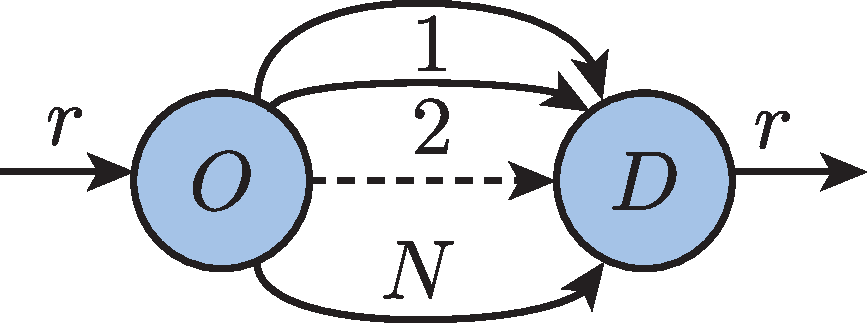
\includegraphics[height=0.5in]{\lyxdot \lyxdot /figures/ParLinkNetwork}
\par\end{centering}

\caption{{\footnotesize Network instance $(\NLinks,r)$. $N$ links from $O$
to $D$ with demand $\protect\qdemand$.}}
\label{fig:nparlink}
\end{figure}


We then introduce a cost function, or latency function $l_{n}$, on
each link $n$. A link's cost can be thought of as the latency experienced
by a job assigned to a particular machine $n$ in the case of job
scheduling \cite{roughgarden2001stackelberg}, or the travel time
of a vehicle using a particular road $n$ in the case of traffic assignment.
In a routing game, every non-atomic agent, represented by an infinitesimal
flow, chooses a route in order to minimize her/his individual latency.
\cite{papadimitriou2010new,roughgarden2002bad}.


\subsection{Modeling congestion with latency functions}

To model the effects of queueing on a given link $n$, the latency
$l_{n}$ on the link is typically assumed to be a non-decreasing function
of the amount of flow $x_{n}$ on link $n$ \cite{aswani2011game,babaioff2009congestion,roughgarden2002bad}.
While this class of latency accurately models congestion on a broad
range of networks (such as the internet, and more generally communication
networks), it fails to correctly model congestion for a large class
of networks. For example, consider a link (or road) $n$ in a traffic
network. A given flow $\flow[n]$ may correspond to two different
scenarios: few vehicles on the road are moving quickly (the road is
in \emph{free-flow}), in which case the latency on the road is low,
or a large number of vehicles on the road are moving slowly (the road
is \emph{congested}), in which case the latency on the road is high.
This phenomenon is not captured if the latency is only a function
of flow, as such functions do not allow capacity to decrease as latencies
increase (Figure~\ref{fig:example-flow-latency} shows how mapping
flow to latency is not unique). One way to address this limitation
is to have two latency functions: one describes the latency on a link
\emph{in free-flow}, while the other describes the latency on a link
\emph{in congestion. }Equivalently, one may introduce a second binary
argument $m_{n}\in\left\{ 0,1\right\} $ to the latency function,
designed to specify whether the link is in free-flow or in congestion.

We next show that such latency functions can be derived from macroscopic
models of flow on horizontal queuing networks.


\subsection{Deriving latency functions for horizontal queuing networks\label{sub:Deriving-a-Class}}

The relationship between the speed of flow on a network and the \emph{density}
of flow (or amount of flow in the static sense) is usually expressed
by a function called the flux function in the physical sciences and
conservation law theory and fundamental diagram in traffic flow theory
\cite{daganzo1994cell,papageorgiou1989macroscopic}. Figure \ref{fig:permfds}
depicts a triangular flux function, while similarly shaped diagrams
have been developed for certain applications.

While such flow models have been popular for many decades in specific
domains (such as traffic and fluid mechanics), less attention has
been given to these models in the literature studying routing games,
which focuses on modeling latency as a non-decreasing function of
flow, and assumes flow and density to have a one-to-one relation.
In order to characterize Nash equilibria on horizontal queues, we
develop a novel approach based on the unique structure of the latency
functions.

Consider a link $\link$ with length $\Length[\link],$ and assume
the flow $\flow[n]$ on the link is given by a function:\vspace{-0.10in}
\begin{align*}
x_{n}^{\rho}:D_{n} & \rightarrow\Rea_{+}\\
\rho_{n} & \mapsto x_{n}=x_{n}^{\rho}(\rho_{n})
\end{align*}
 The function $x_{\link}^{\rho}$ maps density $\rho_{n}$ to flow,
is defined on the domain $D_{n}\subset\Rea_{+}$, and corresponds
to the fundamental diagram of traffic%
\footnote{\label{fn:papa}Note, this allows for fundamental diagrams with unbounded
density support, for example as in \cite{papageorgiou1989macroscopic}:
$\flow\left(\mass\right)=\mass e^{-\mass}$ %
}. The latency is given by a function:\vspace{-0.10in} 
\begin{align*}
\latency[\link]^{\rho}:D_{n} & \rightarrow\Rea_{+}\\
\rho_{n} & \mapsto l_{n}^{\rho}(\rho_{n})
\end{align*}


We observe that latency is related to flow and density through the
relation:\vspace{-0.10in}

\begin{equation}
\latency[\link]^{\mass}\left(\mass[\link]\right)=\frac{\Length[\link]\mass[\link]}{x_{n}^{\rho}\left(\mass[\link]\right)},\label{eq:latency-relation}
\end{equation}


We make three assumptions on the flow and latency functions $x_{n}^{\rho}$
and $l_{n}^{\rho}$ for horizontal queues, which are illustrated in
Figure \ref{fig:permfds}.
\begin{enumerate}
\item There exists a critical density $\masscrit[\link]>0$, such that the
latency is constant and minimal on the interval $\left[0,\masscrit[n]\right]$.
This is equivalent to the flow function $\flow[\link]^{\rho}$ being
linear on that interval.
\item $x_{n}^{\rho}$ is maximal at $\masscrit[\link]$. The value of the
flow at critical density is denoted $\flowMax[\link]=x_{n}^{\rho}(\masscrit[\link])$
and referred to as maximum flow or \emph{capacity} of the link.
\item The latency function $\latency[\link]^{\rho}$, is continuous, non-decreasing.\vspace{-0.05in}
\begin{figure}
\begin{centering}
\subfloat[{\footnotesize Fundamental diagram examples.\label{fig:Fundamental-diagram-examples.}}]{\begin{raggedright}
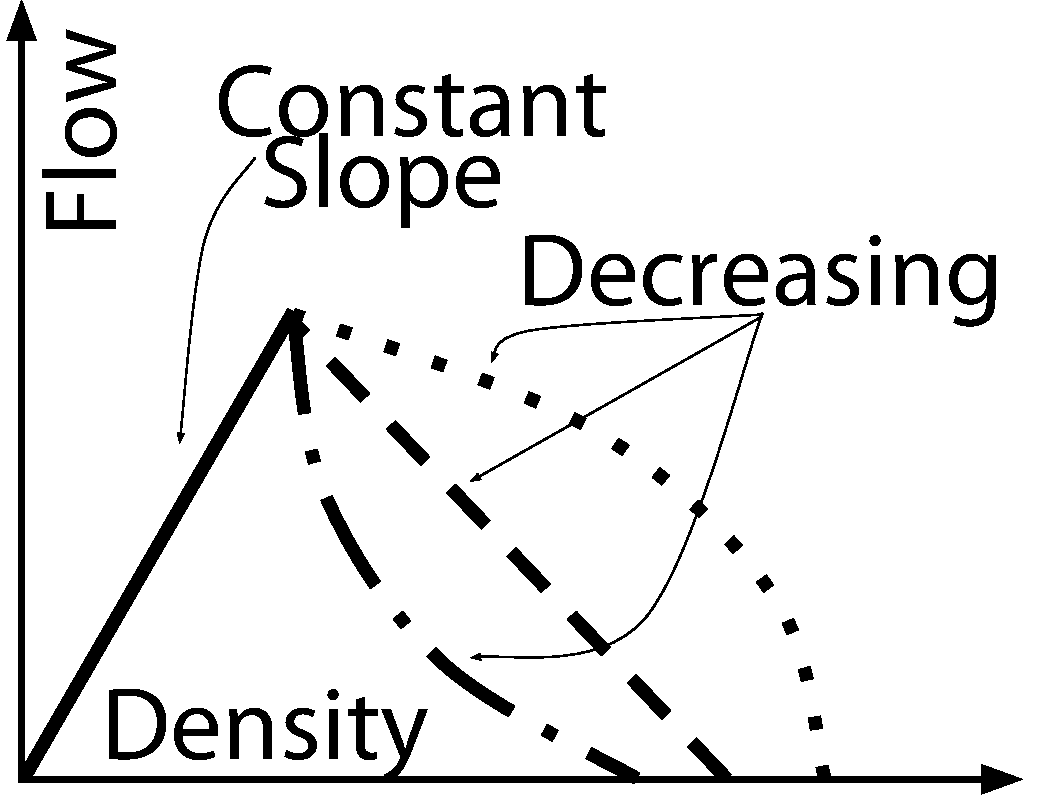
\includegraphics[height=0.75in]{\lyxdot \lyxdot /figures/AnnotatedFundamentalDiagramMatched}
\par\end{raggedright}

\label{fig:permfds}}$\quad$\subfloat[{\footnotesize Latency as a function of density examples.\label{fig:example-rho-latency}}]{\begin{raggedright}
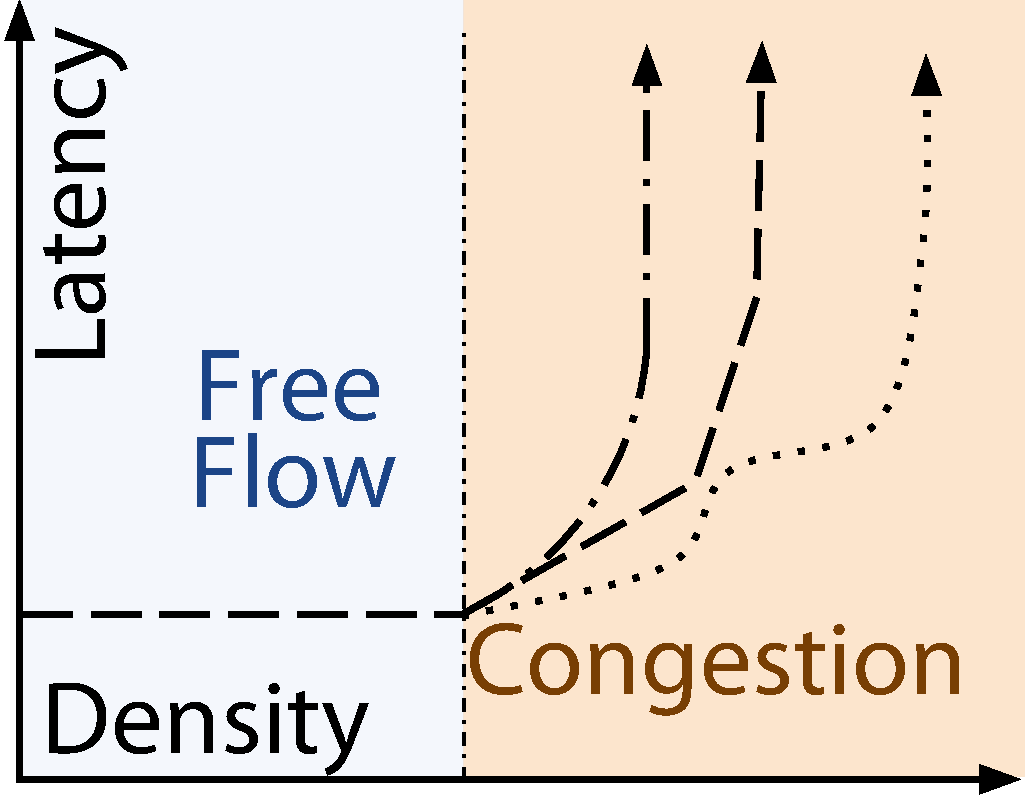
\includegraphics[height=0.75in]{\lyxdot \lyxdot /figures/LatencyasFunctionofDensityMatched}
\par\end{raggedright}

\raggedright{}}$\quad$\subfloat[{\footnotesize Latency as a function of flow and state.\label{fig:example-flow-latency}}]{\begin{raggedright}
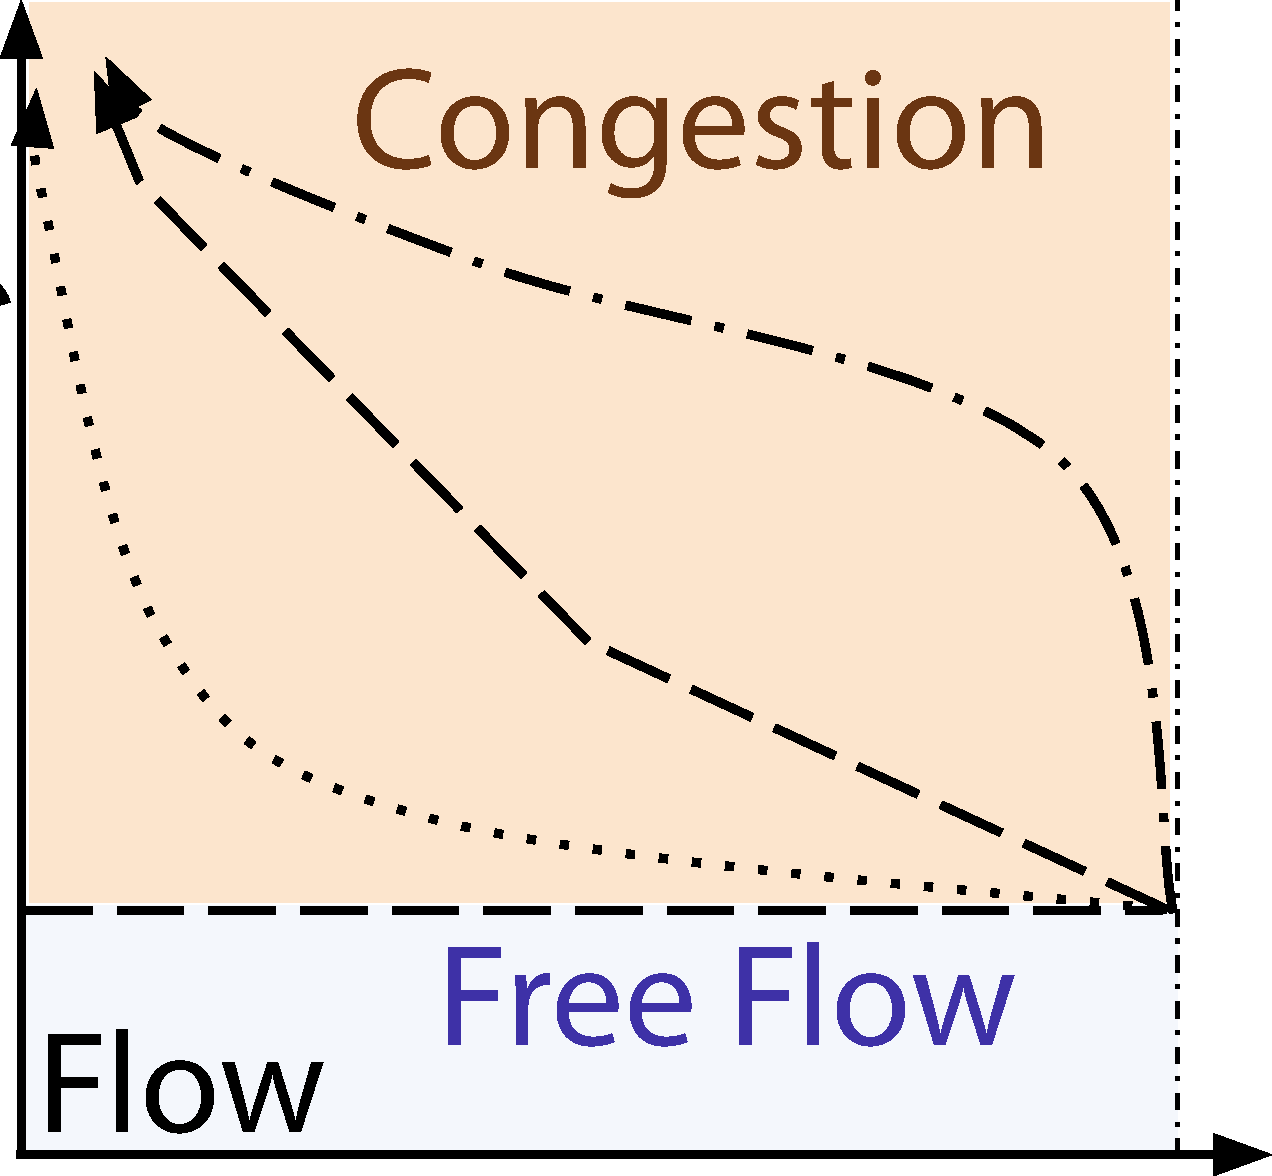
\includegraphics[height=0.75in]{\lyxdot \lyxdot /figures/LatencyasFunctionofFlowModeMatched}
\par\end{raggedright}

\raggedleft{}}
\par\end{centering}

\caption{{\footnotesize Examples of flux functions and corresponding latency
functions that satisfy the assumptions in Section \ref{sub:Deriving-a-Class}.
The dotted line describes a flux function which reacts less severely
to increasing density than the dashed and dot-dashed lines.}}
\end{figure}

\end{enumerate}
We define the \emph{free-flow region} as $\mass[\link]\in\left[0,\masscrit[\link]\right]$
and \emph{congested region} as $\mass[\link]>\masscrit[\link]$. These
assumptions define a class of supported fundamental diagrams. Assumption
2 just states that $\forall\mass[\link]\ge0$, $\flow[\link]^{\rho}\left(\mass[\link]\right)\in\left[0,\flowMax[\link]\right]$.
From Equation \eqref{eq:latency-relation}, Assumption 3 can be expressed
equivalently in terms of the flow function $x_{n}^{\rho}$ as $\frac{d\flow[\link]^{\rho}\left(\mass[\link]\right)}{d\mass[\link]}\le\frac{x_{n}^{\rho}\left(\mass[\link]\right)}{\mass[\link]}$.
This gives reasonable restrictions on the shape of fundamental diagrams
in the congestion region, and flexible enough to allow non-concavity,
and even increasing functions $\flow[\link]^{\rho}$ under certain
conditions. Examples of allowable fundamental diagrams are given in
Figure \ref{fig:permfds}, and corresponding examples of latency functions
are given in Figure \ref{fig:example-rho-latency}. Note that from
these assumptions, we can write the latency function for the horizontal
queueing model as:\vspace{-0.10in}

\[
\latency[\link]^{\mass}\left(\mass[\link]\right)=\begin{cases}
\frac{\Length[\link]\masscrit[\link]}{\flowMax[\link]} & \mass[\link]\in\left[0,\masscrit[\link]\right]\\
\frac{\Length[\link]\mass[\link]}{\flow[\link]\left(\mass[\link]\right)} & \textup{otherwise}
\end{cases}
\]

\begin{example}
\emph{Triangular fundamental diagrams}

One particular class of fundamental diagrams $x^{\rho}$ that satisfy
the above assumptions are triangular fundamental diagrams \cite{daganzo1994cell},
which are linear with positive slope $\speedff$ in the free-flow
region, affine with negative slope $\speedCong$ in the congestion
region, and have maximum flow $\flowMax=\masscrit\speedff$. Assumptions
1 and 2 are satisfied by definition, and Assumption 3 is satisfied
since $\frac{d\flow\left(\mass\right)}{d\mass}=\speedff=\frac{x\left(\mass\right)}{\mass}$
$\forall\rho\in[0,\masscrit]$ and $\frac{d\flow\left(\mass\right)}{d\mass}=\speedCong\le0\le\frac{x\left(\mass\right)}{\mass}$
$\forall\rho\geq\masscrit$. The dotted line in Figure \ref{fig:Fundamental-diagram-examples.}
shows a triangular fundamental diagram. The latency function is then
given by:\vspace{-0.10in}

\[
\latency[\triangle]^{\mass}\left(\mass\right)=\begin{cases}
\frac{\Length}{\speedff} & 0\le\mass\le\frac{\flowMax}{\speedff}\\
\frac{\Length\mass}{\speedCong\left(\mass-\massmax\right)} & \frac{\flowMax}{\speedff}<\mass\le\massmax
\end{cases}
\]


where $\massmax=\flowMax\left(\frac{1}{\speedff}-\frac{1}{\speedCong}\right)$.
\end{example}

\subsection{A class of latency functions for horizontal queues}

\label{sub:latency_class}

While expressing latency as a function of density is intuitive and
succinct for horizontal queues, expressing it as a function of flow
proves to be more convenient in the study of congestion games. This
is largely due to the fact that total flow must be conserved in traffic
assignment problems, and not density. For this reason, we introduce
an equivalent formulation of latency using flow and a binary argument
that describes congestion state. Let the congestion state $\Mode[\link]$
of link $\link$ be defined as:\vspace{-0.10in}

\[
\Mode[\link]:=\begin{cases}
0 & \text{if }\link\text{ is in free-flow}\\
1 & \text{if }\link\text{ is congested}
\end{cases}
\]
We can now define a general class of latency functions $\latency[\link]$
as a function of both flow and congestion state:\vspace{-0.20in}

\begin{align*}
\latency[\link]:\left[0,\flowMax[\link]\right]\times\left\{ 0\right\} \cup(0,\flowMax[n])\times\left\{ 1\right\}  & \rightarrow\Rea_{+}\\
\left(\flow[\link],\Mode[\link]\right) & \mapsto\latency[\link]\left(\flow[\link],\Mode[\link]\right),
\end{align*}


Note that the latency in congestion $l_{n}(\cdot,1)$ is defined on
the open interval $(0,\flowMax[n])$. In particular, if $\flow[n]=0$
then $m_{n}=0$ (an empty link is in free-flow) and if $\flow[n]=\flowMax[n]$
then $\Mode[n]=0$ (if a link is at maximum capacity, it is considered,
by convention, to be in free-flow. It is in fact on the boundary of
the free-flow and congestion regions, and we choose this convention
to simplify the discussion). We also assume that $\latency[\link]$
satisfies the following properties, which are equivalent to the assumptions
in Section~\ref{sub:Deriving-a-Class}:
\begin{itemize}
\item The latency in free-flow is constant. Equivalently, $\forall\flow[n]\in[0,\flowMax[n]]$,
$\latency[\link]\left(\flow[\link],0\right)=\parA[\link]$, where
$a_{n}$ is the constant free-flow latency.
\item $\lim_{\flow[n]\rightarrow\flowMax[\link]}\latency[\link]\left(\flow[n],1\right)=\latency[\link]\left(\flowMax[\link],0\right)=a_{n}$
\item $x\mapsto\latency[\link]\left(x,1\right)$ is decreasing on $(0,\flowMax[n])$.
\end{itemize}
When $\Mode[\link]=1$, the latency $\latency[\link]$ may be unbounded
as the flow decreases to zero. Some examples of latency functions
in this class are illustrated in Figure \ref{fig:example-flow-latency}.
Again, the latency function corresponding to a triangular fundamental
diagram can be readily expressed in this form:\vspace{-0.15in}

\begin{align*}
\latency[\triangle]\left(x,0\right) & =\frac{\Length}{\speedff}\\
\latency[\triangle]\left(\flow,1\right) & =L\left(\frac{\massmax}{\flow}+\frac{1}{\speedCong}\right)
\end{align*}
\vspace{-0.20in}


\subsection{Total System Cost}

The cost to an agent is defined as the latency experienced by the
agent, or the latency of the link chosen by the agent. Therefore,
the total cost experienced on a particular link $C_{\link}\left(\flow[\link],\Mode[\link]\right)=\latency[\link]\left(\flow[\link],\Mode[\link]\right)\flow[\link]=\Length[\link]\mass[\link]$.
Then, the total system cost is the sum of the costs of the individual
links $C\left(\flow,\Mode\right)=\sum_{n=1}^{\NLinks}C_{n}\left(\flow[n],\Mode[n]\right)$,
where $\flow=(x_{1},\dots,x_{\NLinks})$ is the vector of flows, and
$\Mode=(m_{1},\dots,m_{\NLinks})$ is the vector of congestion states
for the entire network.


\section{Nash Equilibria\label{sec:Nash-Equilibria}}

In this section, we characterize pure non-atomic Nash equilibria of
the network (also called Wardrop equilibria in the transportation
literature), which we simply refer to as Nash equilibria. We show
that our class of latency functions induce multiple Nash equilibria
with different costs, and that the set of Nash equilibria can be computed
in polynomial time (with respect to the number of parallel links).
Then we characterize the best Nash equilibrium and focus our attention
on studying the inefficiency of the best Nash equilibrium in Section~\ref{sec:Inefficiency}.


\subsection{Characterization of Nash Equilibria}

We first recall the fundamental notion of Nash equilibrium for the
network instance $(\NLinks,r)$ \cite{roughgarden2002bad,papadimitriou2010new}.
\begin{definitn}
\emph{Nash Equilibrium}

\label{def:ne}An assignment $(\flow,\Mode)\in\Rea[\NLinks]_{+}\times\{0,1\}^{\NLinks}$
for the network instance $(\NLinks,\qdemand)$ is a Nash equilibrium,
if $\forall n$ 
\[
\flow[\link]>0\Rightarrow\forall k\leq N,\ \latency[\link](\flow[\link],\Mode[\link])\leq\latency[k](\flow[k],\Mode[k])
\]

\end{definitn}
In particular, every non-atomic agent cannot improve her/his latency
by switching to another link. As a consequence, all links that are
in the support of $\flow$ have the same latency $\latency[0]$, and
links that are not in the support have latency greater than or equal
to $\latency[0]$. We will denote by $\Supp{\flow}$ the support of
$\flow$, i.e. the set $\left\{ n\in\left\{ 1,\dots,\NLinks\right\} |\flow[n]>0\right\} $.

Note that to fully describe the equilibrium, one needs to specify
the congestion state vector $m$ in addition to the flow assignment
$x$, since the latency on a link depends on whether the link is congested
or not. The following Lemma gives an equivalent characterization of
Nash equilibria.
\begin{lemma}
\emph{Characterization of a Nash Equilibrium}

\label{lem:nash_eq} A feasible assignment $(\flow,\Mode)$ for a
network instance $(\NLinks,\qdemand)$ is a Nash equilibrium if and
only if $\exists\: l_{0}>0$ such that\vspace{-0.10in} 
\begin{align*}
\flow[\link]>0 & \Rightarrow\latency[\link](\flow[\link],\Mode[\link])=\latency[0]\\
\flow[\link]=0 & \Rightarrow\latency[\link](0,0)\geq\latency[0]
\end{align*}
 The total latency incurred by the network is $\Latency(\flow,\Mode)=\qdemand\latency[0]$.
\end{lemma}
Note that links that have zero flow are necessarily in free-flow $\flow[\link]=0\Rightarrow\Mode[\link]=0$.


\subsection{\label{sub:Traffic-Networks-Have} Multiple Nash equilibria on networks
with horizontal queues}

Let $\NashEquilibrium{\NLinks}{\qdemand}{}$ denote the set of Nash
Equilibria for network instance $(\NLinks,r)$. For our class of latency
functions, the essential uniqueness property of Nash equilibrium \cite{roughgarden2002bad}
does not hold.%
\footnote{Note that essential uniqueness of Nash Equilibria holds for the class
of non decreasing latency functions, i.e. all Nash Equilibria have
the same cost. To show this result, assume that the latency functions
$\flow[\link]\mapsto\latency[\link](\flow[\link])$ are non-decreasing
and only depend on the flow $\flow[n]$. Let $\flow$ and $\flow'$
be two Nash equilibria for $(\NLinks,\qdemand)$. Let $\latency[0]$,
respectively $\latency[0]'$ denote the common latency of all links
in the support of $\flow$, respectively $\flow'$. The cost of the
Nash equilibria are respectively $\qdemand\latency[0]$ and $\qdemand\latency[0]'$.
Assume $\flow\neq\flow'$. Then $\exists\link_{1},\link_{2}$ such
that $\flow[\link_{1}]>\flow[\link_{1}]'\geq0$ and $\flow[\link_{2}]'>\flow[\link_{2}]\geq0$.
Since $\flow$ is at Nash equilibrium and $\link_{1}\in\Supp{\flow}$,
$\latency[\link_{1}](\flow[\link_{1}])\leq\latency[\link_{2}](\flow[\link_{2}])$.
And since $\latency[\link_{2}]$ is non-decreasing $\latency[\link_{2}](\flow[\link_{2}])\leq\latency[\link_{2}](\flow[\link_{2}]')$.
Thus $\latency[0]=\latency[\link_{1}](\flow[\link_{1}])\leq\latency[\link_{2}](\flow[\link_{2}])\leq\latency[\link_{2}](\flow[\link_{2}]')=\latency[0]'$.
Exchanging the roles of $\flow$ and $\flow'$ we have $\latency[0]'\leq\latency[0]$.
Therefore $\latency[0]=\latency[0]'$ and both equilibria have the
same cost.%
} To see this, consider for example a network instance $(\mbox{\ensuremath{\NLinks}=}2,\mbox{\ensuremath{\qdemand}=}1)$
where $\flowMax[1]=\flowMax[2]=1$, the free-flow latencies are $a_{1}=1$
and $a_{2}=2$, and the congested latency functions are given respectively
by $l_{1}(\flow[1],1)=\frac{1}{x_{1}}$ and $l_{2}(\flow[2],1)=\frac{2}{x_{2}}$.
Then it is easy to see that $(x,m)=((1,0),(0,0))$, $(x',m')=((\frac{1}{2},\frac{1}{2}),(1,0))$,
and $(x'',m'')=((\frac{1}{3},\frac{2}{3}),(1,1))$ are all Nash equilibria
for this instance, and they have different costs: $C(x,m)=1$, $C(x',m')=2$
and $C(x'',m'')=3$. This simple example shows that there are at least
two types of Nash equilibria: equilibria for which every link in the
support is congested (this is the case for $(x'',m'')$ in the previous
example), and equilibria that have one link in free-flow in their
support (this is the case for both $(x,m)$ and $(x',m')$). In this
section, we show that these are in fact the only possible types of
equilibria, and we prove that there are at most $2\NLinks$ such equilibria,
assuming free-flow latencies are distinct. To simplify the discussion,
we assume without loss of generality, that the links are ordered by
increasing free-flow latencies, and that free-flow latencies are different
to avoid degenerate cases where the set of Nash equilibria is infinite:
\begin{quote}
\emph{Assumption:}\textbf{ }($\parA[1]<\parA[2]<\ldots<\parA[\NLinks]$).
\end{quote}
We start by deriving properties that the congestion state vector $m$
needs to satisfy for a Nash equilibrium $(x,m)$.
\begin{lemma}
\emph{Congestion of lower links}

\label{lem:filluplower}Let $\left(\flow,\Mode\right)\in\NashEquilibrium{\NLinks}{\qdemand}{}$. 

Then $j\in\Supp{\flow}\Rightarrow\Mode[i]=1\quad\forall i\in\left\{ 1,\ldots,j-1\right\} $\end{lemma}
\begin{proof}
Let $i\in\left\{ 1,\ldots,j-1\right\} $. Then $\Mode[i]=0\Rightarrow\latency[i](x_{i,}m_{i})=\parA[i]<a_{j}\le\latency[j](x_{j},m_{j})$,
which violates the characterization of Nash equilibrium in \prettyref{lem:nash_eq}.
Therefore, $m_{i}=1\quad\forall i\in\left\{ 1,\ldots,j-1\right\} $.\end{proof}
\begin{cor}
\emph{Congestion states under equilibrium}

\label{cor:atmost1ff} Let $\left(\flow,\Mode\right)\in\NashEquilibrium{\NLinks}{\qdemand}{}$.
Assume that $\exists j\in\Supp{\flow}$ such that $m_{j}=0$. Then
$m=(1,\dots,\stackrel{j-1}{1},\stackrel{j}{0},\dots,0)$ and $\Supp{\flow}=\left\{ 1,\dots,j\right\} $.\end{cor}
\begin{proof}
We have from Lemma \ref{lem:filluplower} that $\forall i\in\left\{ 1,\dots,j-1\right\} $,
$m_{i}=1$. And we have $\forall i\in\left\{ j+1,\dots,N\right\} $,
$l_{i}(x_{i},m_{i})\geq a_{i}$ by definition of the latency function,
and $a_{i}>a_{j}$ since $i>j$. Therefore the latency on link $i\in\left\{ j+1,\dots,N\right\} $
is strictly greater than the latency on link $j\in\Supp x$, therefore
$i\notin\Supp x$ (follows from the characterization of Nash equilibrium
in Lemma \ref{lem:nash_eq}) and $m_{i}=0$.
\end{proof}
The corollary states that if some link $j$ in the support of a Nash
equilibrium is in free-flow, this completely determines the congestion
state vector of the equilibrium: links $\left\{ 1,\dots,j-1\right\} $
are in the support and are congested, and links $\left\{ j+1,\dots,N\right\} $
are not in the support. We will call such Nash equilibria (where a
single link in the support is in free-flow) \emph{single link free-flow
equilibri}a. In general a Nash equilibrium does not necessarily have
a link in free-flow: this defines a second type of equilibria where
all links in the support are congested, i.e. $m_{\max\Supp x}=1$.
We will call such equilibria \emph{congested equilibria}.

The following Lemma shows that given a congestion state vector $m$,
there are at most two corresponding Nash equilibria $(x,m)$, one
single link free-flow equilibrium, and one congested equilibrium.
\begin{lemma}
\emph{Enumerating Nash Equilibria}

\label{lem:enumerate_nash_eq}For a given congestion state $\Mode$,
there are at most two assignments $x$ such that $(x,m)$ is a Nash
equilibrium.\end{lemma}
\begin{proof}
Let $m\in\left\{ 0,1\right\} ^{N}$ be a given congestion state vector
and assume $x,x'\in\Rea[\NLinks]_{+}$ are such that $(x,m)$ and
$(\flow',m)$ are two different Nash equilibria. Then $\exists i,j$,
$1\leq i<j\leq N$ such that $0\leq\flow[i]<\flow[i]'$ and $0\leq\flow[j]'<\flow[j]$
(we assume without loss of generality that $i<j$: if this is not
the case, exchange $\flow$ and $\flow'$). 

We start by noting that since $j\in\Supp{\flow}$ and $i<j$, then
$i\in\Supp{\flow}$. This follows from the fact that $l_{i}(0,m_{i})=a_{i}<a_{j}\leq l_{j}(\flow[j],m_{j})$,
thus if $j\in\Supp{\flow}$, $\flow[i]$ cannot be zero since every
link in the support of a Nash equilibrium has latency $\le$ the latency
on any other link. 

Now since $i,j\in\Supp{\flow}$, then we have $l_{i}(x_{i},m_{i})=l_{j}(\flow[j],m_{j})$.
And since $j\in\Supp{\flow}$ and $i<j$, then by \prettyref{lem:filluplower},
we have $m_{i}=1$ (link $i$ is congested). Therefore $\latency[i](x_{i},m_{i})>\latency[i](x'_{i},m_{i})$
since $l_{i}(.,1)$ is decreasing. Finally we have $\latency[j](x_{j},m_{j})\leq\latency[j](x'_{j},m_{j})$
since $l_{j}(.,0)$ is constant and $\latency[j](.,1)$ is decreasing.
Combining the above, we have\vspace{-0.20in}

\begin{equation}
\latency[i](x'_{i},m_{i})<l_{i}(x_{i},m_{i})=\latency[j](x_{j},m_{j})\leq\latency[j](x'_{j},m_{j})\label{eq:contradiction}
\end{equation}
\vspace{-0.20in}

Now we partition the set of Nash Equilibria in two sets $\NashEquilibrium{\NLinks}r{}=\text{NE}_{\text{f}}(\NLinks,r)\sqcup\text{NE}_{\text{c}}(\NLinks,r)$:
equilibria that have a completely congested support, denoted by $\text{NE}_{\text{c}}(\NLinks,r)$,
and equilibria that have one link in free-flow in their support, denoted
by $\text{NE}_{\text{f}}(\NLinks,r)$. Now we show that for a given
congestion state vector $m$, each set contains at most one element.

Suppose $(\flow,m),(\flow',m)\in\NashEquilibrium{\NLinks}{\qdemand}f$,
where $\flow,\flow'$ are as defined above\textbf{.} Then since $j\in\Supp{\flow}$,
we have by \prettyref{lem:filluplower}, $\forall k<j$ $m_{k}=1$.
Since the last link in the support of $\flow'$ is, by assumption,
in free-flow, we have $\max\Supp{\flow'}\geq j$. Therefore $j\in\Supp{\flow'}$.
But from \eqref{eq:contradiction} we have $\latency[i](x'_{i},m_{i})<\latency[j](x'_{j},m_{j})$
which contradicts the definition of a Nash Equilibrium (a link in
the support of a Nash Equilibrium has latency less than or equal to
any other link). Thus there is at most one assignment $x$ such that
$(x,m)\in\NashEquilibrium{\NLinks}{\qdemand}f$.

Suppose $(\flow,m),(\flow',m)\in\NashEquilibrium{\NLinks}{\qdemand}c$,
where $\flow,\flow'$ are as defined above\textbf{.} Then since $j\in\Supp{\flow}$
and every link in the support is congested (by definition of $\NashEquilibrium{\NLinks}{\qdemand}c$),
then $m_{j}=1$. Therefore $ $$j$ is also congested under assignment
$\flow'$, thus $j\in\Supp{\flow'}$. Similarly to the first case,
this leads to a contradiction since $\latency[i](x'_{i},m_{i})<\latency[j](x'_{j},m_{j})$,
which proves that there is at most one assignment $x$ such that $(x,m)\in\NashEquilibrium{\NLinks}{\qdemand}c$.
\end{proof}
This shows that there are at most $2N$ Nash equilibria for the instance
$(\NLinks,r)$: $\NLinks$ single link free-flow equilibria, corresponding
to congestion states $m=(0,\dots,0)$, $m=(1,0,\dots,0)$, $\dots$,
$m=(1,\dots,1,0)$, and $N$ congested equilibria, corresponding to
congestion states $m=(1,0,\dots,0)$, $\dots$, $m=(1,\dots,1)$.
Next, we characterize single link free-flow equilibria.


\subsection{Single link free-flow Equilibria}

Consider a Nash equilibrium $(x,m)$ and let $k=\max\left[\Supp{\flow}\right]$.
Assume $m_{k}=0$ (i.e. $(x,m)$ is a free-flow Nash equilibrium).
We have from Corollary \prettyref{cor:atmost1ff} that links $\left\{ 1,\dots,k-1\right\} $
are congested and link $k$ is in free-flow. Therefore we must have
$\forall n\in\left\{ 1,\dots,k-1\right\} $, $l_{n}(x_{n},1)=l_{k}(x_{k},0)=a_{k}$.
This uniquely determines the flow on congested links $n\in\left\{ 1,\dots,k-1\right\} $.
We define this flow to be $\cffFlow nk$. More precisely,
\begin{definitn}
\emph{Congestion flow}

For $1\leq n<k\leq N$, the congestion flow $\cffFlow nk$ is defined
as the unique flow in $(0,\flowMax[n])$ that satisfies\vspace{-0.10in}

\begin{equation}
l_{n}(\cffFlow nk,1)=a_{k}\label{eq:x_hat}
\end{equation}
\end{definitn}
\begin{prop}
\emph{Congestion Flows are decreasing} 
\begin{equation}
\cffFlow{\link}k=l_{n}(\cdot,1)^{-1}(a_{k})\label{eq:x_hat_alt_def}
\end{equation}
 is a decreasing function of $k$ since $a_{k}$ is increasing in
$k$ and $l_{n}(\cdot,1)^{-1}$ is decreasing.
\end{prop}
We can now characterize single link free-flow equilibria. All single
link free-flow equilibria are of the form $\left(\opneFlow kr,\cffMode k\right)$
where\vspace{-0.25in}

\begin{align}
\bar{\Mode}^{k}\coloneqq(\stackrel{1}{1},\dots,\stackrel{k-1}{1},\stackrel{k}{0},\dots,\stackrel{N}{0})\label{eq:m_bar}\\
\opneFlow k{\qdemand}:=(\overset{1}{\cffFlow 1k},\dots,\overset{k-1}{\cffFlow{k-1}k},r-\sum_{\link=1}^{k-1}\cffFlow{\link}k,0,\dots,\stackrel{\NLinks}{0})\label{eq:x_bar}
\end{align}
\vspace{-0.15in}

Illustrations of Equations \eqref{eq:x_hat}, \eqref{eq:m_bar} and
\eqref{eq:x_bar} are shown in Figure \ref{fig:xbar-and-hat-defns}.
\begin{figure}
\begin{centering}
\subfloat[{\footnotesize Examples of congestion flows $\cffFlow{\link}k$.\label{fig:xhat}}]{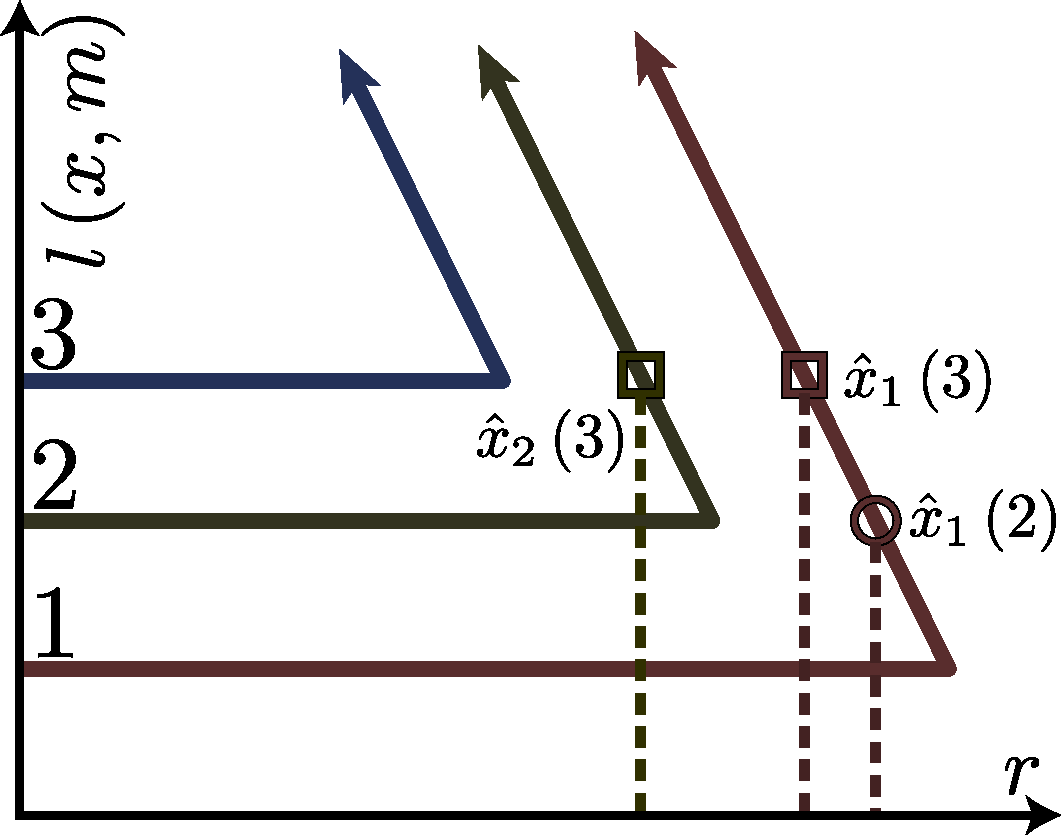
\includegraphics[clip,width=1.6in]{\lyxdot \lyxdot /figures/presentation/DefinitionXHat}}$\quad$\subfloat[{\footnotesize Example of a single link free-flow assignment $(\bar{x}^{3,\qdemand},\bar{m}^{3})$.}]{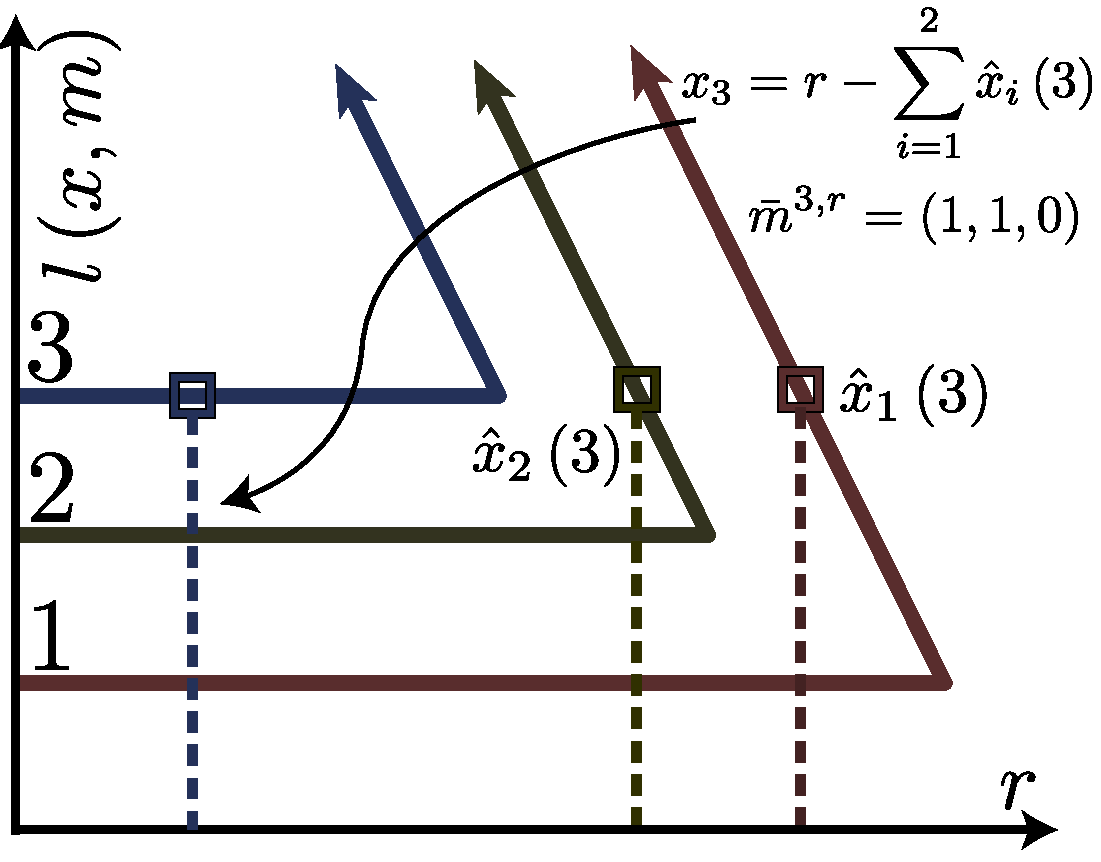
\includegraphics[clip,width=1.6in]{\lyxdot \lyxdot /figures/presentation/DefinitionXBar}}
\par\end{centering}

\centering{}\caption{{\footnotesize Graphical illustration of single link free-flow Nash
equilibria.\label{fig:xbar-and-hat-defns}}}
\end{figure}

\begin{prop}
\emph{Single link free-flow Nash Equilibria}

\label{prop:xbar} If $\bar{x}^{k,r}$ is a feasible assignment, i.e.
$r-\sum_{\link=1}^{k-1}\cffFlow{\link}k\in\left[0,\flowMax[k]\right]$,
then $\left(\opneFlow kr,\cffMode k\right)$ is a Nash Equilibrium
for the instance $(N,r)$.\end{prop}
\begin{proof}
From \prettyref{eq:m_bar} and \prettyref{eq:x_bar}, we have that
$\forall i<k$, $\opneFlow[i]k{\qdemand}\in\left[0,\flowMax[i]\right]$
and $\latency[i](\opneFlow[i]k{\qdemand},\bar{\Mode}_{i}^{k})=\parA[k]$.
And since $\cffMode[k]k=0$ by definition of $\bar{m}_{k}$, we also
have $\latency[k](\opneFlow[k]k{\qdemand},\bar{\Mode}_{k}^{k})=\parA[k]$.
All links $\link>k$ are not in $\Supp{\opneFlow k{\qdemand}},$ and
have a latency greater than $\parA[k]$. Therefore, we have that $\forall\link\in\Supp{\opneFlow k{\qdemand}}$,
$\latency[\link](\opneFlow[n]k{\qdemand},\bar{\Mode}_{n}^{k})=\parA[k]$
and $\forall\link\notin\Supp{\opneFlow k{\qdemand}}$, $l_{n}(\opneFlow[n]k{\qdemand},\bar{\Mode}_{n}^{k})>a_{k}$,
which satisfies the definition of a Nash equilibrium.
\end{proof}

\subsection{Existence of a single-link free-flow Nash Equilibrium}

From Proposition~\prettyref{prop:xbar}, we have a simple characterization
of single link free-flow equilibria. Next, we show that if the set
of Nash equilibria is non-empty, then it contains a single link free-flow
equilibrium.
\begin{lemma}
\emph{Existence of a single link free-flow Nash equilibrium}

\label{lemma:slff}Consider instance $(\NLinks,r)$. If the set of
Nash equilibria is non empty, $\NashEquilibrium{\NLinks}{\qdemand}{}\neq\emptyset$,
then there exists a single link free-flow Nash equilibrium $\left(\opneFlow j{\qdemand},\cffMode j\right)\in\NashEquilibrium{\NLinks}{\qdemand}{}$
for some $j\leq N$.\end{lemma}
\begin{proof}
We first observe that for a network of $\NLinks$ links, the maximum
demand $r$ such that $\NashEquilibrium{\NLinks}r{}\neq\emptyset$
is $\max_{k\in\left\{ 1,\dots,\NLinks\right\} }\left\{ \flowMax[k]+\sum_{\link=1}^{k-1}\cffFlow{\link}k\right\} $.
We denote this quantity with $\maxDemand{\NLinks}$. Therefore, from
\prettyref{lem:filluplower}, it suffices to show the following property: 

$\mathbf{P}_{N}$: $\forall r\in\left[0,\maxDemand{\NLinks}\right]$,
there exists a single link free-flow Nash equilibrium for the instance
$(\NLinks,r)$.

We show $\mathbf{P}_{N}$ by induction on $N$, the size of the network.
For $N=1$, it is clear that if $0\le\qdemand\le\flowMax[1]$, there
is a single-link free-flow equilibrium $(x,m)=(r,0)$. 

Now let $N\geq1$, assume $\mathbf{P}_{N}$ is true and let us show
$\mathbf{P}_{N+1}$. Let $0\leq\qdemand\le\maxDemand{\NLinks+1}$
and consider a network instance $(N+1,r)$. \end{proof}
\begin{case}
If $\qdemand\le\maxDemand{\NLinks}$, then by the induction hypothesis
there exists a single link free-flow Nash equilibrium $(x,m)$ for
the instance $(N,r)$. Then assignment $(x',m')$ defined as $x'=(x_{1},\dots,x_{N},0)$
and $m'=(m_{1},\dots,m_{N},0)$ is clearly a single-link free-flow
Nash equilibrium for the instance $(N+1,r)$.
\end{case}

\begin{case}
If $\maxDemand{\NLinks}<\qdemand\le\maxDemand{\NLinks+1}$ then we
can show that $\left(\opneFlow{N+1}{\qdemand},\cffMode{N+1}\right)\in\NashEquilibrium{\NLinks+1}{\qdemand}{}$.
From Proposition \prettyref{prop:xbar}, we only need to show that\vspace{-0.10in}
\begin{equation}
0\leq\qdemand-\sum_{\link=1}^{N}\cffFlow{\link}{N+1}\leq\flowMax[N+1].\label{eq:ff_existence_need_to_show}
\end{equation}

\end{case}
First, we note that since $\maxDemand{\NLinks}<\maxDemand{\NLinks+1}$,
then $\maxDemand{\NLinks+1}=\flowMax[N+1]+\sum_{\link=1}^{N}\cffFlow{\link}{N+1}$,
thus from $\qdemand<\maxDemand{\NLinks+1}$, we have $r\leq\flowMax[N+1]+\sum_{\link=1}^{N}\cffFlow{\link}{N+1}$
which proves the second inequality of \eqref{eq:ff_existence_need_to_show}.
To show the first inequality, we have \small 
\begin{align*}
r & \ge\flowMax[N]+\sum_{\link=1}^{N-1}\cffFlow{\link}N & \text{since \ensuremath{\maxDemand{\NLinks}}<\ensuremath{\qdemand}}\\
 & \ge\flowMax[N]+\sum_{\link=1}^{N-1}\cffFlow{\link}{N+1} & \text{since }\text{\ensuremath{\cffFlow nN\geq\cffFlow n{N+1}}}\\
 & \geq\cffFlow N{N+1}+\sum_{\link=1}^{N-1}\cffFlow{\link}{N+1} & \text{since }\text{\ensuremath{\flowMax[N]\geq\cffFlow N{N+1}}}
\end{align*}


\normalsize which achieves the induction.
\begin{cor}
\emph{Cost of single link free-flow Equilibria}

\label{cor:ff_eq_better_than_cong_eq}

If there exists a congested equilibrium $(x,m)\in\NashEquilibrium{\NLinks}r{}$,
then there exists a single-link free-flow equilibrium $(x',m')$ with
lower cost.\end{cor}
\begin{proof}
Let $(\flow,\Mode)\in\NashEquilibrium{\NLinks}r{}$ be a congested
equilibrium, i.e. $\Mode[k]=1$ where $k=\max\Supp{\flow}$. Then
we have $r\leq\flowMax[k]+\sum_{\link=1}^{k-1}\cffFlow{\link}k$ and
by the property $\mathbf{P}_{k}$, there exists a single-link free-flow
equilibrium $(\tilde{x},\tilde{m})\in\NashEquilibrium kr{}$, and
the cost of this equilibrium is $C(\tilde{x},\tilde{m})\leq a_{k}r$.
But this also provides a single-link free-flow equilibrium $(x',m')$
for the original instance $(N,r)$ defined by $x'=(\tilde{x}_{1},\dots,\tilde{x}_{k},0,\dots,0)$
and $m'=(\tilde{m}_{1},\dots,\tilde{m}_{k},0,\dots,0)$, and $C(x',m')=C(\tilde{x},\tilde{m})\leq a_{k}r$.
To conclude, we simply note that the cost of the congested equilibrium
is $C(x,m)=l_{k}(x_{k},1)r>a_{k}r$, thus $C(x,m)>C(x',m')$.
\end{proof}

\section{Best Nash Equilibria\label{sec:Best-Nash-Equilibria}}


\subsection{Determining minimum cost Nash equilibria\label{sub:Best-Nash-Equilibria}}

In order to study the inefficiency of Nash equilibria, we focus our
attention on \emph{best Nash equilibria} and \emph{price of stability
}as a measure of their inefficiency (see for example \cite{Anshelevich2004}).
A \emph{best Nash equilibrium} (BNE) is defined to be a Nash equilibrium
of least total latency.
\begin{definitn}
\emph{Best Nash Equilibrium}\label{def:bne}\vspace{-0.10in}
\[
\BestNashEquilibrium{\NLinks}{\qdemand}=\underset{\left(\flow,\Mode\right)\in\NashEquilibrium{\NLinks}{\qdemand}{}}{\arg\min}\Latency\left(\flow,\Mode\right)
\]

\end{definitn}
We now show some interesting properties of the best Nash equilibrium:
\begin{enumerate}
\item $\BestNashEquilibrium{\NLinks}{\qdemand}$ is unique.
\item $\BestNashEquilibrium{\NLinks}{\qdemand}$ is a single-link free-flow
equilibrium.
\item $\BestNashEquilibrium{\NLinks}{\qdemand}$ has the smallest support
of all Nash equilibria for demand $\qdemand$.
\end{enumerate}
These properties are summarized in the following theorem.
\begin{thm}
\emph{Characterization of Best Nash Equilibria}\label{theorem:minsupport}

For a parallel network instance $(\NLinks,r)$, the unique best Nash
equilibrium is the single-link free-flow equilibrium that has smallest
support:\vspace{-0.10in}
\[
\BestNashEquilibrium{\NLinks}{\qdemand}=\underset{\left(\flow,\Mode\right)\in\text{NE}_{\text{f}}(\NLinks,r)}{\arg\min}\left\{ \max\left[\Supp{\flow}\right]\right\} 
\]
\end{thm}
\begin{proof}
From Corollary \prettyref{cor:ff_eq_better_than_cong_eq} we have
that if $(x,m)\in\NashEquilibrium{\NLinks}r{}$ is a congested equilibrium,
then these exists a single-link free-flow equilibrium with lower cost.
Therefore the Best Nash Equilibrium is a single-link free-flow equilibrium.
To show that the BNE has smallest support, we simply note that if
$(x,m)\in\text{NE}_{\text{f}}(\NLinks,r)$ is a single-link free-flow
equilibrium and $k=\max\Supp x$, then its cost is $C(x,m)=a_{k}r$.
Note that uniqueness is immediate since two single-link free-flow
equilibria $(x,m)$ and $(x',m')$ that have the same support, hence
the same congestion state $m=m'$, coincide by \prettyref{lem:enumerate_nash_eq}.
\end{proof}
Theorem \prettyref{theorem:minsupport} therefore provides a simple
characterization of the best Nash equilibrium for any instance $(\NLinks,r)$.
This characterization results in a simple algorithm to compute the
best Nash equilibrium for any network and any feasible demand.


\subsection{Computational complexity of finding Best Nash Equilibria\label{sub:Computational-complexity-of}}

In this section, we present a constructive algorithm for finding the
best Nash equilibrium of a network instance $(\NLinks,r)$ and then
show the running time to be in $O\left(\NLinks^{2}\right)$.

Algorithm \eqref{alg:bestNE} relies on the routine $\texttt{freeFlowConfig}$,
which outputs a candidate \emph{single-link free-flow} assignment
for the instance $(\NLinks,r)$, such that link $i$ is the last link
in the support (Equation \eqref{eq:x_bar}). Starting with link 1
in free-flow, $\texttt{bestNE}$ checks if the output of $\texttt{freeFlowConfig}$
is a feasible assignment. If this is the case, the candidate assignment
is the Best Nash Equilibrium, and $\texttt{bestNE}$ terminates. If
not, the free-flow link index is incremented by one, and the process
is repeated until either a feasible assignment is found, or the number
of links exceeds $\NLinks$, in which case no Nash equilibrium exists.
\begin{algorithm}[h]
\lstinputlisting[basicstyle={\ttfamily \scriptsize},mathescape]{../common-files/algo.raw}

\caption{{\footnotesize Best Nash Equilibrium}}
\label{alg:bestNE}
\end{algorithm}


We first note from Algorithm \prettyref{alg:bestNE} that from the
definition of $\cffFlow ij$, we can precompute $\cffFlow ij\forall1\leq i<j\leq N)$
in $O\left(\NLinks^{2}\right)$. The subroutine $ $$\texttt{freeFlowConfig}$
runs in $O\left(\NLinks\right)$ time. Finally, for each loop of the
$\texttt{bestNE}$ outer routine (with $\NLinks$ iterations), the
running time is a constant plus the running time of $\texttt{freeFlowConfig}$.
Therefore, the overall running time of the algorithm is $O(\NLinks^{2})+\NLinks O(\NLinks)=O(\NLinks^{2})$.


\section{Inefficiency of Best Nash Equilibria\label{sec:Inefficiency}}

To study the inefficiency of Nash equilibria, in particular of the
best Nash equilibrium, we use price of stability as a measure of inefficiency
\cite{Anshelevich2004}. Price of stability is defined as the ratio
between the cost of the best Nash Equilibrium and the social optimal
cost. First we give an overview of social optimum for our model. Then
we consider a simple two link parallel network and derive the price
of stability for a triangular fundamental diagram. We show how this
example illustrates the dependency of the price of stability on the
flow demand and the free-flow latencies.


\subsection{Social Optima\label{sec:Social-Optima}}

Consider an instance $(N,\qdemand)$ where the flow demand $r$ does
not exceed the maximum capacity of the network $r\leq\sum_{n}\flow[\link]^{\max}$.
Since the total cost function is $C(\flow,\Mode)=\sum_{n=1}^{\NLinks}\flow[n]l_{n}(\flow[n],\Mode[n])$,
the social optimum of the network is a solution to the optimization
problem: $\underset{\flow,\Mode}{\min}\sum\flow\latency[\link]\left(\flow[\link],\Mode[\link]\right)$
such that $\sum_{\link}\flow[\link]=\qdemand$. It is shown in \cite{fullversion}
that a socially optimal flow is necessarily in free flow on all links,
which leads to an equivalent linear program: $\underset{\flow,\Mode}{\min}\sum_{\link}\flow[\link]\parA[\link]$
such that $\sum_{\link}\flow[\link]=\qdemand$. Then, since the links
are ordered by increasing free-flow latency $a_{1}<\dots<a_{N}$,
the social optimum is simply given by the assignment that saturates
most efficient links first. Formally, if $k_{0}=\max\{k|r>\sum_{n=1}^{k}x_{n}^{\max}\}$
then the social optimal assignment $x^{*}$ is:\vspace{-0.25in}

\begin{align}
\flow^{*}=(\flowMax[1],\dots,\flowMax[k_{0}],\qdemand-\sum_{n=1}^{k_{0}}\flowMax[n],0,\dots,0)\label{eq:so}
\end{align}
\vspace{-0.30in}


\subsection{Price of Stability on a Two-Link Network\label{sec:Price-of-Stability}}

To characterize the loss of efficiency of Nash equilibria several
metrics have been used including price of anarchy \cite{roughgarden2002bad}
and price of stability \cite{Anshelevich2004}. The price of anarchy
is defined as the ratio between the cost of the \emph{worst} \emph{Nash
equilibrium} and the the social optimum cost, while the price of stability
is defined as the ratio between the \emph{best Nash equilibrium} and
the social optimal cost. For the case of non-decreasing latency functions,
the price of anarchy and the price of stability coincide since all
Nash equilibria have the same cost by the essential uniqueness property
\cite{roughgarden2002bad}. Since we focus our analysis on the best
Nash equilibrium, we use as a metric the price of stability.

Consider a network instance $(2,r)$ such that $\parA[1]<\parA[2]$
and $\flowMax[2]+\cffFlow 12>\flowMax[1]$. Let $\BestNashEquilibrium 2{\qdemand}=\left(\flow[\text{BNE}](r),\Mode[\text{BNE}](r)\right)$
be the best Nash equilibrium and $\left(x_{\text{SO}}(r),0\right)$
be the social optimum, as defined by \prettyref{eq:so}. The price
of stability is then defined as $\POS Nr=\frac{\Latency\left(\flow[\text{BNE}](r),\Mode[\text{BNE}](r)\right)}{\Latency\left(\flow[\text{SO}],0\right)}$.
From social optimum \prettyref{eq:so} and the characterization of
the best Nash equilibrium in Theorem \ref{theorem:minsupport}, we
only need to consider the following two cases:


\paragraph{Case 1: $0\le\protect\qdemand\le\protect\flowMax[1]$}

Using \prettyref{eq:so}, all the demand will be on link 1 in free-flow.
Similarly, from Theorem \prettyref{theorem:minsupport} we have that
since link 1 can accommodate $\qdemand$ in free-flow and the support
cannot be smaller than a single link, then $\BestNashEquilibrium 2{\qdemand}$
has all flow demand on link 1 in free-flow, and is equivalent to the
social optimum. In this case, the price of stability is equal to 1,
i.e there is no decrease in efficiency due to selfish routing.


\paragraph{Case 2: $\protect\flowMax[1]<\protect\qdemand\leq\protect\flowMax[2]+\cffFlow 12$}

We know that all flow demand cannot be accommodated by link 1. From
\prettyref{eq:so}, the social optimum assignment is given by $x_{\text{SO}}(r)=(\flowMax[1],\qdemand-\flowMax[1])$.
From Theorem~\prettyref{theorem:minsupport} we have that $\BestNashEquilibrium 2{\qdemand}$
has a single link in free-flow. Since the total demand exceeds the
capacity of link $1$, then under a best Nash equilibrium, link 2
is in free-flow, and link 1 is congested. Therefore $\Mode[\text{NE}](r)=(1,0)$.
From Algorithm \prettyref{alg:bestNE}, the corresponding flow $\flow[\text{NE}](r)$
will be $(\cffFlow 12,\qdemand-\cffFlow 12)$. The comparison of the
social optimum and Nash equilibrium assignments are depicted in Figure
\ref{fig:sone}.
\begin{figure}
\centering{}\subfloat[{\footnotesize Social optimum\label{fig:Social-optimum}}]{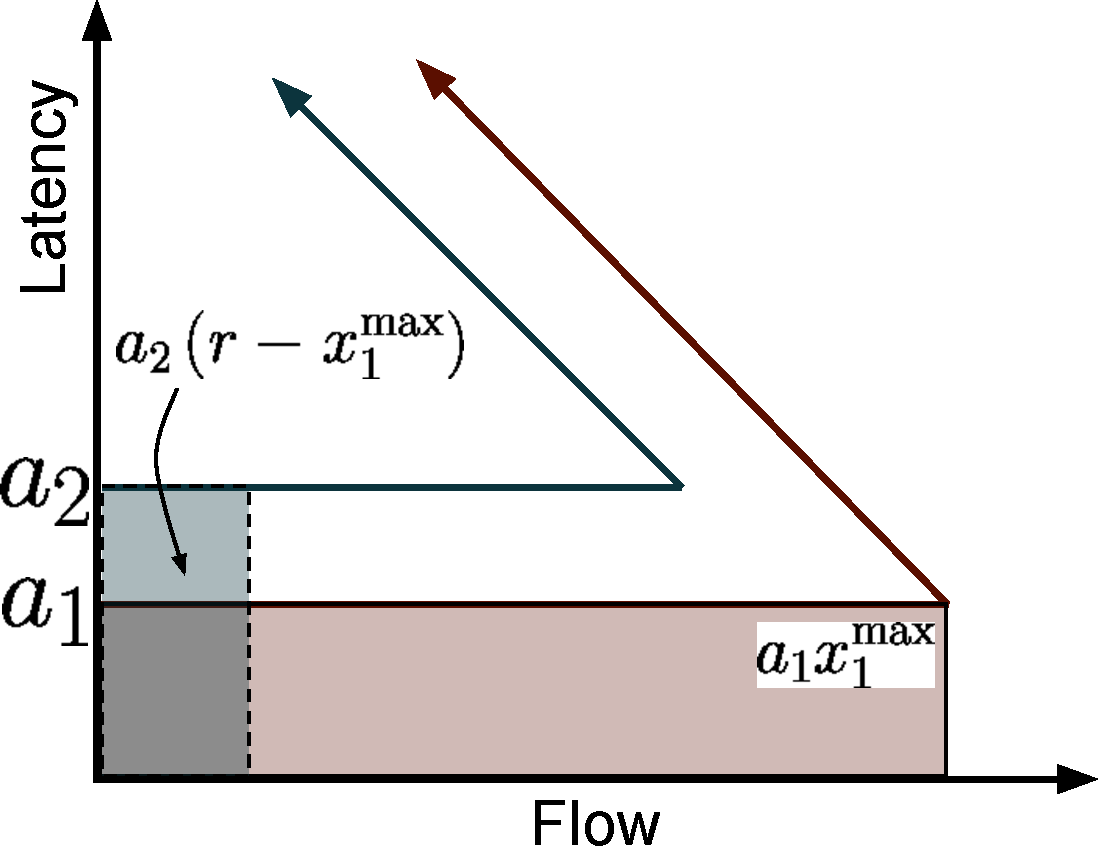
\includegraphics[clip,height=0.9in]{\lyxdot \lyxdot /figures/TwoLinkPOSSO}}\subfloat[{\footnotesize Nash equilibrium\label{fig:Nash-equilibrium}}]{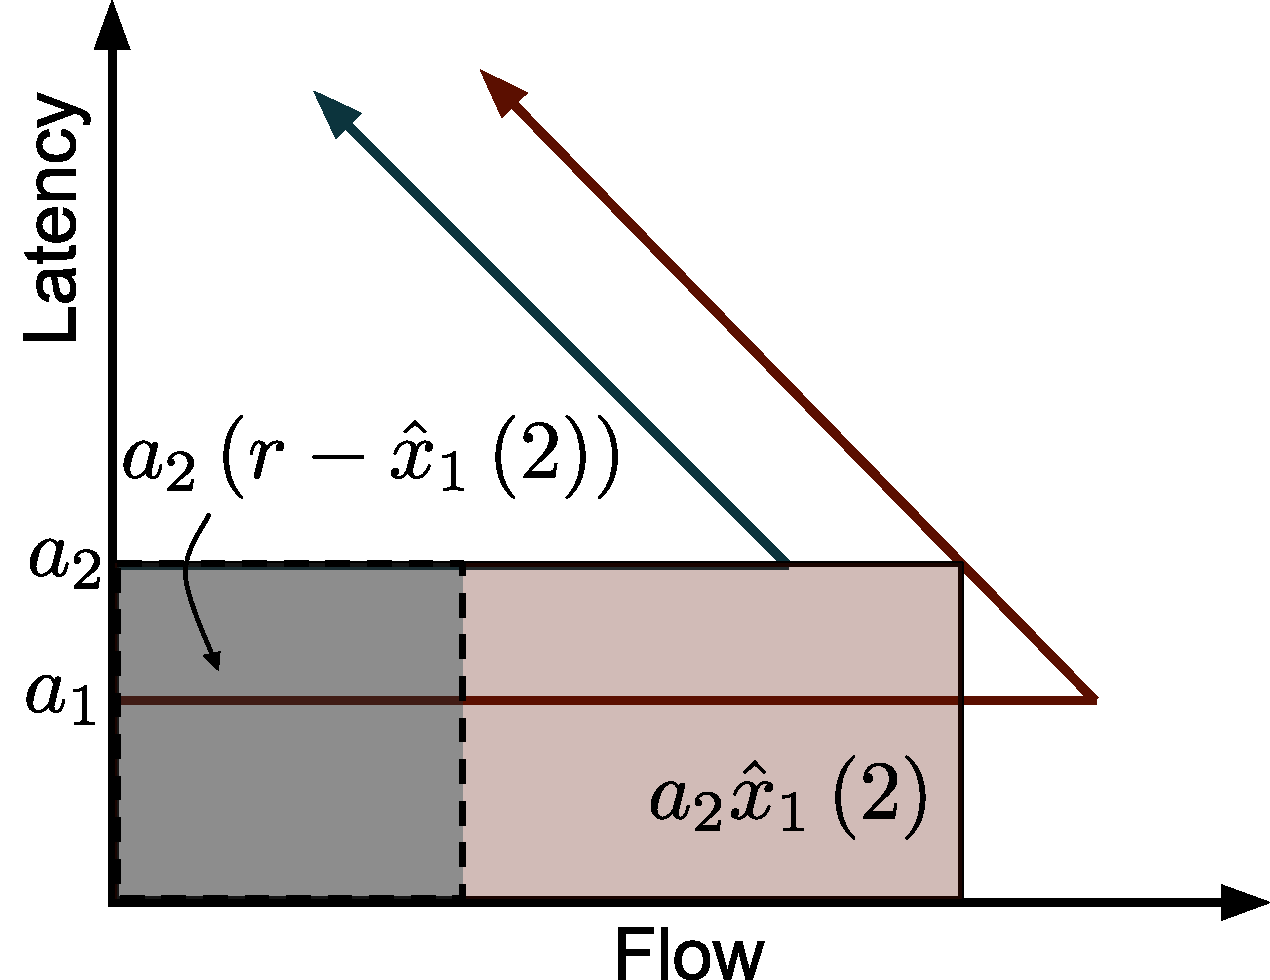
\includegraphics[clip,height=0.9in]{\lyxdot \lyxdot /figures/TwoLinkPOSBNE}}\subfloat[{\footnotesize POS as a function of demand.\label{fig:POS-plot}}]{\raggedright{}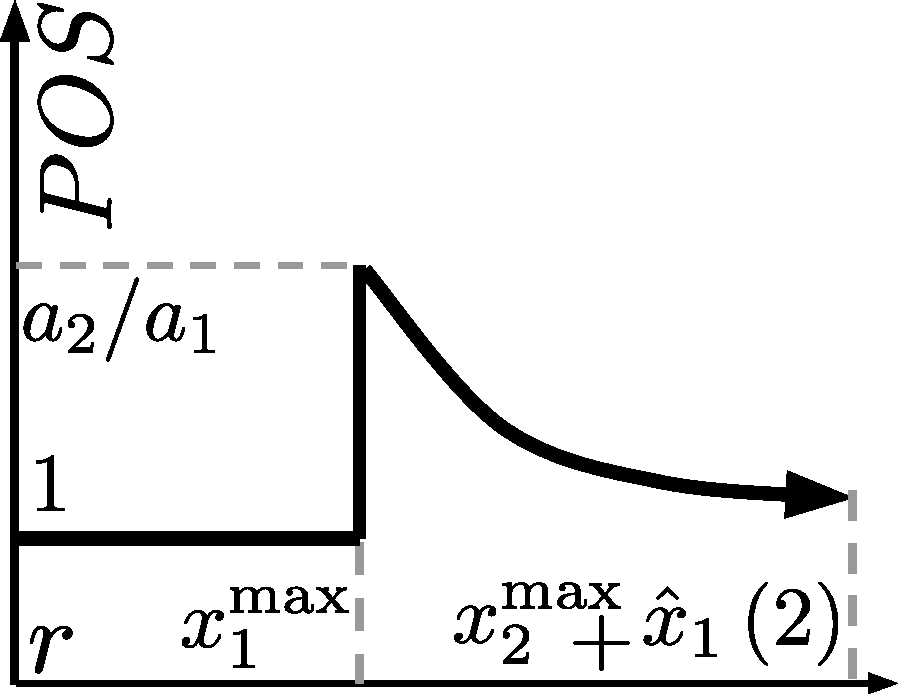
\includegraphics[clip,width=1.1in]{\lyxdot \lyxdot /figures/POSTwoLink}}\caption{{\footnotesize Visualization of POS on two-link network. Differences
in flow assignments between social optimum and Nash equilibrium are
shown in \ref{fig:Social-optimum} and \ref{fig:Nash-equilibrium}.
The area of the shaded regions in \ref{fig:Social-optimum},\ref{fig:Nash-equilibrium}
are the total costs attributed to each link. In \ref{fig:POS-plot},
the flat region corresponds to $\protect\qdemand\le\protect\flowMax[1]$
(Case 1) and the decreasing region to $\protect\qdemand>\protect\flowMax[1]$
(Case 2).}}
\label{fig:sone}
\end{figure}


Computing the price of stability when $\qdemand>\flowMax[1]$ reveals
where the inefficiencies lie in the Nash equilibrium. It is shown
in \cite{fullversion} that $\POS 2{r>\flowMax[1]}=\left(1-\frac{\flowMax[1]}{\qdemand}\left(1-\frac{\parA[1]}{\parA[2]}\right)\right)^{-1}$.
In this simple two-link parallel network, the price of stability is
maximal at $r=\flowMax[1]$ and equal to $\frac{a_{2}}{a_{1}}$ (Figure
\ref{fig:POS-plot}). This shows in particular that for the general
class of horizontal queuing congestion latencies, the price of stability
is unbounded, since for any demand $r$ and any positive constant
$A$, we can design an instance $(2,r)$ such that the price of stability
is $\frac{a_{2}}{a_{1}}>A$.

Also note that for a fixed flow demand $r>\flowMax[1]$, the price
of stability is an increasing function of $\frac{a_{2}}{a_{1}}$.
And as $\parA[2]\rightarrow\parA[1]$, the price of stability goes
to 1. Intuitively, the inefficiency of Nash equilibria can be directly
attributed to the difference in free-flow latency between the links.

Additionally, as the demand $r\geq\flowMax[1]$ increases, the price
of stability decreases. This occurs because the difference in total
latency between social optimum and Nash equilibrium is constant for
$r\geq\flowMax[1]$.

This also shows that selfish routing is most costly when a free-flow
link is near maximum capacity (note the discontinuity in total latency
for Nash equilibrium that occurs when demand exceeds the capacity
of the first link $\qdemand>\flowMax[1]$). If a controller were to
anticipate a scenario where demand was slightly above this capacity,
they could dramatically reduce the inefficiency of the Nash equilibrium
by rerouting a small fraction of the flow and keeping the link in
free-flow.


\section{Conclusion\label{sec:Discussion}}

We introduced a new class of latency functions that models congestion
in horizontal queuing networks, and studied the resulting Nash equilibria
for non-atomic congestion games on parallel networks. We showed the
essential uniqueness property does not hold for this new class, and
that there may be up to $2N$ equilibria for a network instance $(\NLinks,r)$.
Then we focused our attention on the best Nash equilibrium $\BestNashEquilibrium{\NLinks}r$,
which we proved is the single link free-flow equilibrium with smallest
support, and then presented a constructive, quadratic time algorithm
for finding this equilibrium. Finally, we derived price of stability
results for a two-link network, then showed that if a link is anticipated
to be near capacity, congestion can be completely averted by diverting
only a small fraction of the demand.

\bibliographystyle{plain}
\bibliography{../common-files/bibliography}

\end{document}
